\documentclass[11pt]{article}

\usepackage[final]{acl}

\usepackage{times}
\usepackage{latexsym}
\usepackage[T1]{fontenc}
\usepackage[utf8]{inputenc}
\usepackage{microtype}
\usepackage{inconsolata}
\usepackage{graphicx}
\usepackage{booktabs}
\usepackage{amsmath}
\usepackage{xcolor}
\usepackage{fancyvrb}
\usepackage{tikz}
\usetikzlibrary{positioning,arrows.meta}

\newcommand{\pos}{\texttt{<+>}}
\newcommand{\negt}{\texttt{<->}}
\newcommand{\extra}{\texttt{<extra>}}
\newcommand{\arm}[1]{\textsc{#1}}

\title{Retrieved Examples Do Not Help an Error-Typing Process Reward Model,\\
and Showing It Its Own Verdict Tokens Hurts}

\author{Pratik Goyal \\
  Matriculation no.\ 4756040 \\
  {\small\texttt{pratik.goyal@stud.uni-heidelberg.de}} \\\And
  Ashhad Raza Quadri \\
  Matriculation no.\ 4756039 \\
  {\small\texttt{ashhad.quadri@stud.uni-heidelberg.de}} \\\AND
  Institute for Computational Linguistics, Heidelberg University \\
  Seminar on Process Modelling \quad Supervisor: Lei Tang}

\begin{document}
\maketitle

\begin{abstract}
RetrievalPRM improves a binary step grader by showing it similar, already graded solution
steps before it judges a new one. PathFinder-PRM improves the grader differently, by first
asking what kind of error a step contains and only then how good it is. We test whether the
two ideas combine: we insert RetrievalPRM-style references into the prompt of the released
PathFinder-PRM-7B, without any training, and evaluate on ProcessBench. They do not.
Retrieved references with their gold labels lower average F1 from 67.3 to 50.0, and random
references of the same shape lower it to 44.3. Relevance helps a little, and only on the two
hardest subsets, but never enough to offset the loss. Most of the loss comes from how the labels
are written: each reference ends with its judgement in the same \pos{}/\negt{} tokens the model
reads its own verdict from. Writing the identical judgement as the words \emph{correct} and
\emph{incorrect} recovers 12.9 points and is indistinguishable from showing no label at all. A
step-level analysis locates the damage outside the error-typing stage the project set out to
improve: the verdict tokens depress the second stage's correctness score, turning correct steps
into false alarms.
\end{abstract}

\section{Introduction}

A process reward model (PRM) scores each step of a model-generated solution rather than only
its final answer \citep{uesato2022solving,lightman2024verify}. On ProcessBench
\citep{zheng2024processbench}, which asks a grader to locate the first wrong step in a
mathematical solution, two recent 7B systems report strong results by quite different routes.
RetrievalPRM \citep{zhu2025retrievalprm} retrieves questions and steps similar to the one under
judgement from a labelled pool and places them in the prompt, and reports gains that grow with
how far the test problems are from the training distribution. PathFinder-PRM
\citep{pala2025pathfinder} keeps the prompt closed but decomposes the verdict: it first
predicts whether a step contains a \emph{math} error or a \emph{consistency} error, and only
for steps with neither does it estimate a correctness score. It reaches 69.5 average F1
against RetrievalPRM's 65.8.

Neither paper tried the other's idea, and our seminar project asks whether they are
complementary. We address three research questions:
\begin{description}
  \setlength\itemsep{1pt}
  \item[RQ1] Does inserting retrieved references in front of PathFinder-PRM's error-typing
    stage make it better at locating errors, and does any gain grow on more
    out-of-distribution problems, as it does for RetrievalPRM?
  \item[RQ2] Is any change due to the \emph{relevance} of the references, or merely to the
    extra text in the prompt?
  \item[RQ3] Which part of a reference drives the change: the example itself, the judgement
    attached to it, or the form in which that judgement is written?
\end{description}
RQ1 is the question of our project proposal. RQ2 and RQ3 were added as the study developed;
RQ3 arose after the first results and is therefore exploratory.
We kept the setting deliberately narrow. The PathFinder-PRM weights are frozen, the retrieval
recipe follows RetrievalPRM, and the part of the prompt that the model is scored on is
byte-identical in every condition.

The answer to RQ1 is no, but the way it fails turned out to be more interesting than the
question. We ran five arms on the same 200 ProcessBench solutions (\S\ref{sec:setup}), each
differing from another in one respect. Relevant references do slightly better than random ones,
mainly on the hardest subsets, but both lose heavily to no references at all
(\S\ref{sec:results}). The loss is caused mostly by the verdict tokens in which the references'
labels are written, and a step-level analysis places it in PathFinder-PRM's correctness stage
rather than in the error typing we meant to improve (\S\ref{sec:analysis}). Along the way we
found that 59.6\% of ProcessBench's MATH subset appears verbatim in the PathFinder-600K data we
retrieve from, and that a silent encoder fallback had degraded our first retrieval run; both are
described below because both would have changed the conclusions.

\section{Background}
\label{sec:background}

\paragraph{ProcessBench.} ProcessBench \citep{zheng2024processbench} contains 3{,}400
solutions over four sources of increasing difficulty: GSM8K \citep{cobbe2021gsm8k}, MATH
\citep{hendrycks2021math}, OlympiadBench \citep{he2024olympiadbench} and Omni-MATH
\citep{gao2024omnimath}. Each solution is annotated with the index of its first erroneous step,
or $-1$ if it has none. A grader is scored per subset by the harmonic mean of its exact-index
accuracy on erroneous solutions and its accuracy on clean ones. The harmonic mean matters: a
grader that flags everything, or nothing, scores zero.

\paragraph{PathFinder-PRM.} PathFinder-PRM-7B \citep{pala2025pathfinder} is fine-tuned on
PathFinder-600K, a relabelling of PRM800K \citep{lightman2024verify} and automatically annotated
Math-Shepherd-style traces \citep{wang2024mathshepherd}. It uses three special tokens: \pos,
\negt{} and a mask token \extra. The solution so far is placed in the assistant turn, followed
by \textit{``Math reasoning: \extra, Consistency: \extra''}. In stage~1 the model's logits at the
two mask positions are restricted to \pos{} and \negt, and if either is \negt{} the step is
an error. Otherwise stage~2 fills in both verdicts, appends \textit{``, Correctness: \extra''},
runs a second forward pass and takes the softmax probability of \pos{} as the step reward. A
step with reward below $0.5$ is also treated as an error.

\paragraph{RetrievalPRM.} RetrievalPRM \citep{zhu2025retrievalprm} embeds questions and steps
with Sentence-BERT \citep{reimers2019sbert}, reduces the embeddings with PCA and ranks a pool by
cosine similarity, first at question level and then at step level. The retrieved items, each
with its gold label, are added to the prompt as references. The authors argue that question-level
retrieval addresses dataset shift and step-level retrieval addresses differences in reasoning
style, and support this with gains that increase from GSM8K ($+6.4$) to Omni-MATH ($+13.0$).
Their model is trained with references in the prompt; ours is not, which is the main
difference in setting and one we return to in \S\ref{sec:discussion}.

\paragraph{Demonstrations and their labels.} Retrieval of in-context examples by embedding
similarity is known to help large models \citep{liu2022makes}, but it is less clear what the
model uses from them. \citet{min2022rethinking} found that the correctness of demonstration labels
matters surprisingly little for classification, while \citet{zhao2021calibrate} showed that the
label distribution in the prompt biases predictions towards frequent labels. Irrelevant context
also degrades mathematical reasoning \citep{shi2023distracted}. These results frame the failure
modes we test for: extra text that distracts, and labels that bias.

\section{Experimental Setup}
\label{sec:setup}

\begin{figure}[t]
\centering
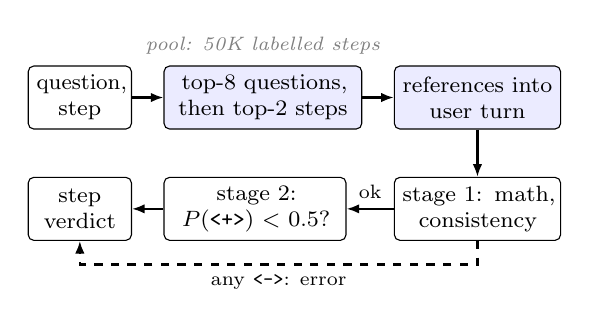
\begin{tikzpicture}[
  font=\footnotesize,
  box/.style={draw, rounded corners=2pt, align=center, inner sep=3pt, minimum height=0.8cm},
  new/.style={box, fill=blue!8},
  arr/.style={-{Latex[length=1.6mm]}, thick}]
\node[box, text width=1.1cm] (q) {question,\\ step};
\node[new, right=0.4cm of q, text width=2.3cm] (r) {top-8 questions,\\ then top-2 steps};
\node[new, right=0.4cm of r, text width=1.9cm] (p) {references into\\ user turn};
\node[box, below=0.6cm of p, text width=1.9cm] (s1) {stage 1: math,\\ consistency};
\node[box, left=0.6cm of s1, text width=2.1cm] (s2) {stage 2:\\ $P(\pos) < 0.5$?};
\node[box, left=0.4cm of s2, text width=1.1cm] (v) {step\\ verdict};
\node[above=0.02cm of r, font=\scriptsize\itshape, text=gray] {pool: 50K labelled steps};
\draw[arr] (q) -- (r);
\draw[arr] (r) -- (p);
\draw[arr] (p) -- (s1);
\draw[arr] (s1) -- node[above, font=\scriptsize] {ok} (s2);
\draw[arr] (s2) -- (v);
\draw[arr, dashed] (s1.south) -- ++(0,-0.3) -| node[pos=0.25, below, font=\scriptsize] {any \negt: error} (v.south);
\end{tikzpicture}
\caption{The system under test. Shaded boxes are what we add to the frozen PathFinder-PRM;
both scoring stages see the same augmented user turn.}
\label{fig:pipeline}
\end{figure}

Figure~\ref{fig:pipeline} shows the system. Everything except the two shaded components is
the released model, used exactly as its authors do.

\subsection{Retrieval}

We follow the RetrievalPRM recipe. The pool is built from the first 50{,}000 parsable step
records of the PathFinder-600K training split: 15{,}316 distinct questions, 21{,}587 steps
from PRM800K and 28{,}413 from the automatically labelled traces. Each record keeps its
question, the step and the step's gold math and consistency labels; 60\% of the steps are
labelled correct on both. Questions and steps are
embedded with all-MiniLM-L6-v2 \citep{wang2020minilm,reimers2019sbert}, projected to 128
dimensions with PCA and L2-normalised, so that cosine similarity is a single matrix product. For
each step to be graded we take the eight most similar pool questions, then rank all steps
belonging to them by similarity to the current step and keep the top two. Each reference is
truncated to 600 characters and any \extra{} tokens in retrieved text are removed, since a stray
mask token would create an additional scoring position.

A contamination guard drops pool questions that are normalised exact duplicates of the test
question or have cosine similarity $\ge 0.95$ to it. The guard is necessary rather than
precautionary. Before running anything we measured overlap between the pool and ProcessBench
(Table~\ref{tab:contamination}). GSM8K, OlympiadBench and Omni-MATH are essentially clean, but
596 of the 1{,}000 MATH questions occur verbatim in the pool, which is expected because PRM800K
was built on MATH. Without the guard, the reference for a MATH item could be a labelled copy of
the very step being judged.

\begin{table}[t]
\centering
\small
\begin{tabular}{lrrr}
\toprule
Subset & $n$ & verbatim & cos $\ge 0.95$ \\
\midrule
GSM8K & 400 & 0 & 0 \\
MATH & 1{,}000 & 596 (59.6\%) & 605 \\
OlympiadBench & 1{,}000 & 0 & 4 \\
Omni-MATH & 1{,}000 & 0 & 24 \\
\bottomrule
\end{tabular}
\caption{Overlap between ProcessBench and our 50K-item retrieval pool. The union, 633
solutions, is excluded in the ``clean'' analyses.}
\label{tab:contamination}
\end{table}

The guard only removes a contaminated item's \emph{neighbours}; the item itself is still graded,
and on MATH it is graded with its second-best references while a clean item gets its best ones.
We therefore report every contrast twice: on all 200 solutions, and on the 173 that remain
after dropping all 633 flagged items from both arms.

\subsection{Prompting}

References go into the user turn only, between PathFinder-PRM's fixed instruction prefix and
the question. The assistant turn, which contains the two mask positions, is identical across
all conditions, and a test compares our prompt strings byte for byte with the example on the
model card. Figure~\ref{fig:prompt} shows the added block. The last line of each reference,
the teacher's judgement, is what distinguishes our treatment and ablation arms.

\begin{figure}[t]
\centering
\fbox{\begin{minipage}{0.94\columnwidth}
\footnotesize\ttfamily
[Reference 1]\\
Question: \textit{\rmfamily (similar pool question)}\\
Step: \textit{\rmfamily (similar pool step)}\\
\textcolor{red!70!black}{Teacher's judgement: Math reasoning: <->, Consistency: <-> (math and consistency error)}\\[3pt]
[Reference 2] \ldots
\end{minipage}}
\caption{The reference block inserted into the user turn (abridged). Arms \arm{B} and \arm{C}
include the red line as shown; arm \arm{E} writes it with \textit{correct}/\textit{incorrect} in
place of \pos/\negt; arm \arm{D} omits it. The assistant turn never changes.}
\label{fig:prompt}
\end{figure}

\subsection{Arms}

The five arms, summarised in Table~\ref{tab:arms}, differ from one another in one configuration
key at a time, and a parity check refuses to compare two runs that differ anywhere else.
\arm{A} is the unmodified model. \arm{B} is the proposed system. \arm{C} replaces the ranked
references with two drawn uniformly from the pool, under the same guard and with the same
rendering, so that \arm{B} and \arm{C} differ only in relevance: \arm{C}'s references have mean
step similarity 0.002 to the step being graded, against 0.479 in \arm{B}. The draw is seeded per
query, so it does not depend on run order. \arm{D} drops the judgement line, and \arm{E} keeps
the same judgement but writes it in words. \arm{B}, \arm{D} and \arm{E} receive identical
references on every step they share, which we verified from the traces.

\begin{table}[t]
\centering
\small
\begin{tabular}{llc}
\toprule
Arm & References (2 per step) & Labels shown \\
\midrule
\arm{A} & none & -- \\
\arm{B} & retrieved (ranked) & \pos/\negt \\
\arm{C} & random from pool & \pos/\negt \\
\arm{D} & retrieved (ranked) & none \\
\arm{E} & retrieved (ranked) & as words \\
\bottomrule
\end{tabular}
\caption{Experimental arms. \arm{C}$\to$\arm{B} isolates relevance; \arm{D}$\to$\arm{B}
isolates the labels; \arm{E}$\to$\arm{B} isolates the verdict tokens at fixed information.}
\label{tab:arms}
\end{table}

\paragraph{A retrieval bug, found and corrected.} Our first run of \arm{B} did not use
Sentence-BERT. A Windows security policy was blocking a library that \texttt{sentence-transformers}
depends on, and our code fell back to a hand-written encoder meant to reproduce it. That fallback
omitted the final normalisation step: its vectors pointed in the right direction but were about
5.8 times too long, so after the PCA projection, which is fitted on unit vectors, retrieval
returned poor neighbours (in one checked case, those ranked 760th and 3{,}333rd). We noticed only
because \arm{E}'s references, produced later with the real encoder, did not match \arm{B}'s. We
fixed the fallback, added a test that compares it with Sentence-BERT directly, and re-ran \arm{B}.
\arm{C} was run under the same fallback but draws its references at random; recomputing them with
the corrected encoder reproduces all 732 of its steps exactly. Every \arm{B} number in this paper
comes from the corrected run. The degraded first run scored 46.3, below the corrected 50.0, which
is itself weak evidence that relevance matters.

\subsection{Evaluation}

\paragraph{Sample.} Full ProcessBench runs were out of reach (see below), so we evaluate 50
solutions per subset, 200 per arm, and the same 200 in every arm. The sample is stratified by
whether a solution contains an error and drawn with a fixed seed. We learned this the hard
way: ProcessBench lists all erroneous solutions of a subset before the first clean one, so our
first 92-minute pilot, which took the first $n$ rows, contained no clean solutions and left F1
undefined on every subset. The stratified sample preserves each subset's own ratio (26/24
erroneous/clean on GSM8K, 38/12 on Omni-MATH).

\paragraph{Statistics.} Per-subset F1 differences are too noisy at $n=50$ to test on their own,
so the main quantities are the change in macro-averaged F1, with a 95\% paired bootstrap interval
over 2{,}000 resamples drawn within subsets \citep{efron1993bootstrap}, and a McNemar test on
solution-level correctness pooled over all 200 solutions \citep{mcnemar1947,dror2018hitchhiker}.
We treat a McNemar result as reliable only with at least 25 discordant solutions.

\paragraph{Inference.} All experiments ran on a single consumer laptop, an Acer Nitro 16S AI
with an NVIDIA GeForce RTX 5070 Laptop GPU (8\,GB of VRAM). The bf16 model
needs about 15\,GB, and disk offloading cost roughly 100\,s per solution, so we quantised the
weights to int4 (group size 64) with torchao, keeping the embedding and output layers in bf16:
the verdict is a comparison of two output logits, and quantising the head would add noise to
exactly the quantity we measure. All arms use the same precision, so differences between
arms are comparable, but absolute scores should not be compared to bf16 results. Early stopping
halts a solution at its first flagged step. One more practical note: the model card loads the
checkpoint with \texttt{AutoModel}, which in current versions of the Transformers library
\citep{wolf2020transformers} returns hidden states without the language-model head; we load it
as a causal LM instead, which is what the card's scoring code assumes.

\paragraph{Compute budget.} The five reported arms together took about 17 GPU hours, from 55
minutes for \arm{A} to about five and a half hours for \arm{E}. Including pilot runs, failed
attempts, the discarded first run of \arm{B}, building the retrieval index and the contamination
check, the project used about 40 hours of compute on this machine. The reference-carrying arms
are slower because their prompts are longer (about 840 tokens against 350 for \arm{A});
retrieval itself accounts for only about 1\% of the time per step. The longest Omni-MATH
solutions exceed the 8\,GB of VRAM: memory spills into shared system RAM, a single step can take
around 24 seconds, and one run of \arm{E} failed with an out-of-memory error. Because every
solution is written to disk as soon as it is scored, interrupted runs were resumed without
recomputing or changing any finished solution. These costs are what limited the study to 200
solutions per arm.

\section{Results}
\label{sec:results}

\paragraph{The baseline reproduces.} Arm \arm{A} reaches 67.3 average F1
(Table~\ref{tab:main}), close to the 69.5 reported by \citet{pala2025pathfinder} over the full
benchmark at bf16. With 50 solutions per subset and int4 weights we did not expect a closer
match, and the ordering of the subsets is as expected, with Omni-MATH hardest. We take this as
evidence that our adapter is faithful, which every comparison below depends on.

\begin{table}[t]
\centering
\small
\setlength{\tabcolsep}{4.5pt}
\begin{tabular}{lrrrrr}
\toprule
 & GSM8K & MATH & Olymp. & Omni & Avg. \\
\midrule
\arm{A} & 70.0 & 72.7 & 69.8 & 56.8 & \textbf{67.3} \\
\arm{E} & 69.0 & 66.5 & 63.7 & 52.5 & 62.9 \\
\arm{D} & 65.7 & 61.6 & 63.7 & 52.5 & 60.9 \\
\arm{B} & 55.1 & 50.3 & 49.0 & 45.7 & 50.0 \\
\arm{C} & 54.1 & 54.3 & 34.5 & 34.2 & 44.3 \\
\midrule
\multicolumn{5}{l}{PathFinder-PRM, published (bf16, full)} & 69.5 \\
\multicolumn{5}{l}{RetrievalPRM, published (bf16, full)} & 65.8 \\
\bottomrule
\end{tabular}
\caption{ProcessBench F1 for each arm (int4, 50 solutions per subset, same solutions in every
arm). Published averages are included for orientation only.}
\label{tab:main}
\end{table}

\paragraph{RQ1: retrieval hurts, on every subset.} Adding retrieved, labelled references lowers
average F1 by 17.3 points, with the bootstrap interval well away from zero
(Table~\ref{tab:contrasts}). The pooled McNemar test is lopsided: 43 solutions that \arm{A}
gets right and \arm{B} gets wrong, against 8 in the other direction. The loss appears on all
four subsets ($-14.9$, $-22.4$, $-20.8$ and $-11.1$ from GSM8K to Omni-MATH), with no trend
across difficulty in either direction.

\paragraph{RQ2: relevance helps a little, where RetrievalPRM says it should.} Random references
cost 23.0 points, retrieved ones 17.3. The difference, \arm{C}$\to$\arm{B}, is $+5.8$ with an
interval of $[-1.1, +12.8]$ ($p=0.10$ over 46 discordant solutions), and $+2.3$ on clean data.
Averaged over the benchmark, relevance therefore has at most a modest effect, and the interval
excludes gains much above RetrievalPRM's largest ones. The per-subset picture is more
interesting. On GSM8K and MATH relevance changes nothing ($+1.0$, $-4.0$), while on
OlympiadBench and Omni-MATH, the two hardest and uncontaminated subsets, it adds $+14.4$
($[+1.2, +29.0]$) and $+11.6$ ($[+0.0, +27.1]$). That is the shape of RetrievalPRM's result.
We treat it as suggestive only: these are two per-subset intervals among many, both barely clear
zero, and in neither subset does relevance make up for the loss relative to \arm{A}.

\paragraph{RQ3: the verdict tokens carry most of the loss.} Arm \arm{D} sees the same
references as \arm{B} without the judgement line and scores 60.9, so \arm{D}$\to$\arm{B} is
$-10.8$ ($[-17.8, -4.7]$, 32 against 8 discordant, $p<0.001$), about two thirds of the total
loss. Arm \arm{E} separates the judgement from its form. It shows exactly the same judgements as
\arm{B}, written as \emph{correct}/\emph{incorrect}, and scores 62.9: \arm{E}$\to$\arm{B} is
$-12.9$ ($[-19.0, -7.7]$, 33 against 6 discordant, $p<0.0001$), and $-17.0$ on clean data. By
contrast, \arm{D}$\to$\arm{E} is $+2.0$ ($[-2.2, +6.4]$). Knowing the judgement costs nothing
measurable; reading it in the model's own verdict tokens costs 11 to 13 points. What remains is
the cost of the reference text itself: \arm{A}$\to$\arm{D} is $-6.5$ and \arm{A}$\to$\arm{E}
$-4.4$, but both rest on about 20 discordant solutions and their clean-data intervals include
zero, so we regard them as a possible small cost rather than an established one.

\begin{table}[t]
\centering
\small
\setlength{\tabcolsep}{3.5pt}
\begin{tabular}{lrcrr}
\toprule
 & $\Delta$F1 & 95\% CI & disc. & $\Delta$F1 clean \\
\midrule
\arm{A}$\to$\arm{B} & $-17.3$ & $[-25.2, -10.1]$ & 8/43 & $-18.8$ \\
\arm{A}$\to$\arm{C} & $-23.0$ & $[-31.2, -15.4]$ & 7/54 & $-21.1$ \\
\arm{C}$\to$\arm{B} & $+5.8$ & $[-1.1, +12.8]$ & 29/17 & $+2.3$ \\
\arm{A}$\to$\arm{D} & $-6.5$ & $[-12.8, -1.5]$ & 5/16$^\dagger$ & $-5.7$ \\
\arm{D}$\to$\arm{B} & $-10.8$ & $[-17.8, -4.7]$ & 8/32 & $-13.1$ \\
\arm{A}$\to$\arm{E} & $-4.4$ & $[-10.0, +0.6]$ & 4/12$^\dagger$ & $-1.7$ \\
\arm{D}$\to$\arm{E} & $+2.0$ & $[-2.2, +6.4]$ & 9/6$^\dagger$ & $+4.0$ \\
\arm{E}$\to$\arm{B} & $-12.9$ & $[-19.0, -7.7]$ & 6/33 & $-17.0$ \\
\bottomrule
\end{tabular}
\caption{Paired contrasts on macro-average F1. ``disc.'' gives the discordant solutions as
(second arm right only / first arm right only). ``Clean'' drops the 27 contaminated solutions
from both arms ($n=173$); in row order the clean intervals are $[-27.9,-9.9]$,
$[-31.0,-13.1]$, $[-6.2,+11.2]$, $[-13.0,+0.3]$, $[-21.9,-5.3]$, $[-7.0,+3.7]$, $[-1.9,+10.6]$
and $[-25.1,-10.7]$. $^\dagger$Fewer than 25 discordant pairs.}
\label{tab:contrasts}
\end{table}

\section{Where the Damage Happens}
\label{sec:analysis}

A drop in F1 can come from missed errors, from false alarms, or from errors found at the wrong
step. Table~\ref{tab:profile} separates these over the 200 shared solutions. With verdict-token
labels, the rate at which clean solutions are flagged rises from 16.4\% to 34--40\%, and among
erroneous solutions the flag moves earlier: the mean difference between predicted and gold index
goes from $+0.32$ to $-0.63$ in \arm{B}, and the share flagged before the true error rises from
12\% to 38\%. The only number that improves is the miss rate, which is what one would expect
from a grader whose effective threshold has been lowered. Arms \arm{D} and \arm{E} stay close to
\arm{A}: they raise somewhat more false alarms, but they do not move the flag earlier, and their
exact-index accuracy is almost unchanged.

\begin{table}[t]
\centering
\small
\setlength{\tabcolsep}{2.6pt}
\begin{tabular}{lrrrrr}
\toprule
 & \arm{A} & \arm{D} & \arm{E} & \arm{B} & \arm{C} \\
\midrule
clean flagged & 16.4 & 26.0 & 23.3 & 34.2 & 39.7 \\
errors missed & 10.2 & 11.0 & 13.4 & 9.4 & 7.9 \\
exact if flagged & 65.8 & 62.8 & 65.5 & 46.1 & 38.5 \\
flagged too early & 12.3 & 15.9 & 13.6 & 38.3 & 49.6 \\
mean index offset & $+0.32$ & $+0.12$ & $+0.24$ & $-0.63$ & $-1.03$ \\
\bottomrule
\end{tabular}
\caption{Solution-level verdict profile in percent, except the offset (predicted minus gold
index). Clean-solution figures are over the 73 clean solutions, the rest over the 127 erroneous
ones.}
\label{tab:profile}
\end{table}

Our hypothesis going in was that references would change stage~1, the error typing, since that
is where they were meant to help. The step-level traces show otherwise. We restrict the
comparison to the 629 steps that were scored in all five arms (early stopping means later steps
are not always reached), of which 548 precede the gold error or belong to clean solutions and
so should not be flagged. Figure~\ref{fig:stages}(a) splits the false flags on these steps by the
stage that raised them. Stage~1 false flags stay between 2.0\% and 2.6\% in every arm, and the
overall stage-1 flag rate barely moves (7.8\% in \arm{A}, 8.4\% in \arm{B}, 7.6\% in \arm{C}).
The increase comes almost entirely from stage~2: 0.4\% of correct steps are rejected by the
correctness score in \arm{A}, against 8.0\% in \arm{B} and 11.5\% in \arm{C}. A bootstrap that
resamples whole solutions (185 of them, since steps of one solution are not independent) puts
the stage-2 increase at $+7.7$ points for \arm{B} (95\% CI $[+5.4, +10.5]$) and $+11.1$ for
\arm{C} ($[+8.4, +14.5]$), while the stage-1 changes, $+0.5$ ($[-0.6, +1.8]$) and $+0.4$
($[-0.3, +1.1]$), are indistinguishable from zero. Figure~\ref{fig:stages}(b) shows why: among
steps that pass stage~1, the whole distribution of $P(\pos)$ moves down when verdict tokens are
in the prompt (mean 0.92 in \arm{A}, 0.79 in \arm{B}), so that 8.5\% of them fall below the
$0.5$ threshold, against 0.3\% in \arm{A}. With the judgement written in words the shift nearly
disappears (\arm{E}: mean 0.87, 1.0\% below threshold, stage-2 increase $+0.7$, $[+0.0, +1.7]$).

\begin{figure}[t]
\centering
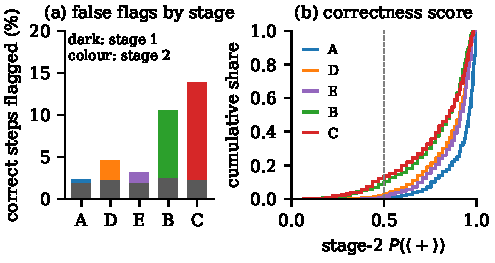
\includegraphics[width=\columnwidth]{figures/stages.pdf}
\caption{(a) Share of gold-correct steps flagged as erroneous, split by the stage that flagged
them. (b) Cumulative distribution of the stage-2 correctness probability for steps that passed
stage~1; the dashed line is the decision threshold. Both panels use the 629 steps scored in all
five arms.}
\label{fig:stages}
\end{figure}

The same pattern holds at solution level. Of the 140 solutions that \arm{B} flags, 57 are
flagged by the correctness score alone, with both error types predicted as absent; in \arm{C}
this holds for 77 of 146, in \arm{E} for 11 of 127, and in \arm{A} for 6 of 126. The additional
flags in the verdict-token arms are mostly not typed errors at all. The typing itself changes
only slightly: consistency errors are predicted a little more often in \arm{B} (4.6\% of steps
against 3.0\% in \arm{A}), too little to account for the F1 loss.

We also checked whether better retrieval limits the damage. Splitting \arm{B}'s solutions into
three equal bins by mean reference similarity (0.39, 0.48 and 0.56) gives accuracy losses
relative to \arm{A} of 20.9, 19.7 and 11.9 points. The best-matched third loses least, in line
with the small relevance effect above, but it is also the bin where \arm{A} itself does worst
(56.7\% against 71.6\% and 75.8\%), so it simply has less to lose.

\section{Discussion}
\label{sec:discussion}

The results rule out the simplest version of our hypothesis. For a frozen PathFinder-PRM,
references do not help, and the difficulty pattern that supported RetrievalPRM appears only
faintly, inside a contrast between two arms that both perform far below the baseline. We see
three reasons why this is compatible with RetrievalPRM's findings.

First, the verdict tokens are not neutral text for this model. \pos{} and \negt{} are the two
tokens whose logits define every verdict it gives, and in arms \arm{B} and \arm{C} four of them
appear in the user turn of every query. Our code already guarded against the mask token \extra{}
leaking into retrieved text; we did not anticipate that the verdict tokens could be equally
disruptive. Arm \arm{E} shows that it is the tokens and not the information: the same judgements
in words are harmless. The direction of the effect is also informative. A majority-label bias of
the kind described by \citet{zhao2021calibrate} would push the model towards \pos, since 60\% of
pool steps are labelled correct on both dimensions, yet we observe a shift towards \negt, and it
is confined to the graded stage-2 decision rather than the two hard stage-1 decisions. Simple
label copying therefore does not explain it. Our reading is that verdict tokens in the context
disturb the calibration of the one logit comparison that is used as a probability rather than
an argmax. RetrievalPRM, a binary grader trained with its references, has no such
second-stage score to disturb.

Second, RetrievalPRM trains its grader with references in the prompt, so the model learns how
to use them. PathFinder-PRM has only ever seen its own fixed prompt. The small, uncertain cost
of unlabelled or word-labelled references ($-4$ to $-7$ points) and the modest value of
relevance fit a model that tolerates extra context but was never taught to exploit it. That the
relevance effect is concentrated on the hardest subsets suggests the signal RetrievalPRM relies
on is there, and a model fine-tuned with references might be able to use it.

Third, error typing may simply be the part of PathFinder-PRM least in need of help. Stage~1 did
not measurably change under any intervention we tried, while the continuous correctness score
was fragile. If references are to be useful to a hierarchical grader, they may have to be
restricted to the stage they are meant to inform, which the current prompt format does not
allow, since both stages share the same user turn.

For anyone building on this, three methodological points generalise beyond our setting. A
retrieval arm without a length-matched random control would have attributed the whole loss to
retrieval. Retrieval pools derived from PRM800K overlap heavily with ProcessBench's MATH subset,
which is exactly where a RetrievalPRM-style hypothesis predicts moderate gains; an unguarded pool
could manufacture those gains from memorisation \citep{sainz2023contamination}. And silent
fallbacks are dangerous: our degraded encoder produced plausible numbers and was caught only
because a later arm's references failed to match. Logging which retrieval path actually ran, and
checking that arms meant to share references really do, is cheap insurance.

\section{Conclusion}

We combined RetrievalPRM-style references with the frozen PathFinder-PRM-7B. On \textbf{RQ1},
the answer is negative: references lower ProcessBench F1 by 17 points, on every subset. On
\textbf{RQ2}, relevance has a modest effect at most, $+5.8$ points on average and not
significant, although it is concentrated on the two hardest subsets, in the pattern RetrievalPRM
reported. On \textbf{RQ3}, the loss is caused mainly by the form of the labels: the same
judgements written as words cost nothing measurable, while written as the model's own verdict
tokens they cost 11 to 13 points, by depressing the correctness score of the second stage rather
than by changing the error typing we set out to improve. The most useful follow-ups are a bf16
replication on the full benchmark and a version of the model fine-tuned with references, which
would test the idea under the conditions in which RetrievalPRM was shown to work. Code,
configurations and all predictions are in our project repository.

\section*{Limitations}

We could not measure whether the predicted error \emph{types} are correct. ProcessBench
annotates only the index of the first erroneous step, not whether the error concerns the
mathematics or consistency with earlier steps. Our evaluation of RQ1 therefore rests on how well
the grader locates errors, and our statements about the error-typing stage (\S\ref{sec:analysis})
describe how often it flags steps, not how accurately it classifies them. Answering the
proposal's original question about error-type accuracy would require a benchmark with gold
error types, or a manually annotated sample.

All results are at int4 precision on 200 of the 3{,}400 ProcessBench solutions. Differences
between arms are valid because every arm used the same weights and sample, but the absolute
scores are not comparable to published bf16 numbers, and per-subset figures carry intervals of
roughly $\pm$15 points and should be read as shape rather than evidence; this applies in
particular to the per-subset relevance effect in \S\ref{sec:results}. We tested one retrieval
configuration: two references per step, one encoder, a 50K-item pool taken from the start of
PathFinder-600K rather than sampled from all of it, and one guard threshold. Sensitivity checks
at other thresholds and with more references were planned but not run. Arms \arm{D} and \arm{E}
were designed after we had seen the first results, so the label findings are exploratory in the
strict sense, although the size and consistency of the effect make chance an unlikely
explanation. Finally, the step-level analysis uses only steps reached in all five arms, which
over-represents early steps.

Most of these limitations come from compute. With a single 8\,GB laptop GPU, one arm on
200 solutions already takes up to five and a half hours, and a full-benchmark run of all five
arms would take roughly 290 hours, about twelve days of continuous computation, extrapolating
from our measured time per solution.

What is missing is hardware, not implementation. Our code already contains everything needed
for the larger study: bf16 configurations for every arm, a full-benchmark mode that simply omits
the sample limit, and configuration switches for the sensitivity checks (guard threshold,
number of references, and question-only retrieval without the step-level stage). With a GPU of
24\,GB or more these could be run as they are. Running at bf16 would make absolute scores
comparable to the published ones, the full 3{,}400 solutions would narrow the per-subset
intervals considerably and settle whether relevance really helps on the hardest subsets, and the
sensitivity checks would show whether our findings depend on the one retrieval configuration we
tested. The only experiment that would need new code is a version of PathFinder-PRM fine-tuned
with references in its prompt. More compute would make the results more precise, more complete
and more general; we would not expect it to reverse the main findings, since the key contrasts
are already far outside their confidence intervals.

\section*{Use of AI Assistants}

We used an AI assistant (Claude, via Claude Code) during this project to help debug and fix our
implementation, for example when tracing library and environment errors and the encoder
fallback described in \S\ref{sec:setup}, to help write analysis scripts, and to help draft and
edit parts of this report. The research questions, the experimental design, the
choice of controls and the running of all experiments are our own. Every number in the paper
was produced by our code and checked by us against the committed result files, and we take
full responsibility for the content of this report.

\section*{Acknowledgements}

We thank Lei Tang for supervising the project and for feedback on the proposal.

\bibliography{references}

\end{document}
